\documentclass[]{article}
\usepackage{lmodern}
\usepackage{amssymb,amsmath}
\usepackage{ifxetex,ifluatex}
\usepackage{fixltx2e} % provides \textsubscript
\ifnum 0\ifxetex 1\fi\ifluatex 1\fi=0 % if pdftex
  \usepackage[T1]{fontenc}
  \usepackage[utf8]{inputenc}
\else % if luatex or xelatex
  \ifxetex
    \usepackage{mathspec}
  \else
    \usepackage{fontspec}
  \fi
  \defaultfontfeatures{Ligatures=TeX,Scale=MatchLowercase}
\fi
% use upquote if available, for straight quotes in verbatim environments
\IfFileExists{upquote.sty}{\usepackage{upquote}}{}
% use microtype if available
\IfFileExists{microtype.sty}{%
\usepackage{microtype}
\UseMicrotypeSet[protrusion]{basicmath} % disable protrusion for tt fonts
}{}
\usepackage[margin=1in]{geometry}
\usepackage{hyperref}
\hypersetup{unicode=true,
            pdftitle={Data Analysis for TechPointX Xbot Digital Assistant},
            pdfauthor={Dante Razo},
            pdfborder={0 0 0},
            breaklinks=true}
\urlstyle{same}  % don't use monospace font for urls
\usepackage{color}
\usepackage{fancyvrb}
\newcommand{\VerbBar}{|}
\newcommand{\VERB}{\Verb[commandchars=\\\{\}]}
\DefineVerbatimEnvironment{Highlighting}{Verbatim}{commandchars=\\\{\}}
% Add ',fontsize=\small' for more characters per line
\usepackage{framed}
\definecolor{shadecolor}{RGB}{248,248,248}
\newenvironment{Shaded}{\begin{snugshade}}{\end{snugshade}}
\newcommand{\AlertTok}[1]{\textcolor[rgb]{0.94,0.16,0.16}{#1}}
\newcommand{\AnnotationTok}[1]{\textcolor[rgb]{0.56,0.35,0.01}{\textbf{\textit{#1}}}}
\newcommand{\AttributeTok}[1]{\textcolor[rgb]{0.77,0.63,0.00}{#1}}
\newcommand{\BaseNTok}[1]{\textcolor[rgb]{0.00,0.00,0.81}{#1}}
\newcommand{\BuiltInTok}[1]{#1}
\newcommand{\CharTok}[1]{\textcolor[rgb]{0.31,0.60,0.02}{#1}}
\newcommand{\CommentTok}[1]{\textcolor[rgb]{0.56,0.35,0.01}{\textit{#1}}}
\newcommand{\CommentVarTok}[1]{\textcolor[rgb]{0.56,0.35,0.01}{\textbf{\textit{#1}}}}
\newcommand{\ConstantTok}[1]{\textcolor[rgb]{0.00,0.00,0.00}{#1}}
\newcommand{\ControlFlowTok}[1]{\textcolor[rgb]{0.13,0.29,0.53}{\textbf{#1}}}
\newcommand{\DataTypeTok}[1]{\textcolor[rgb]{0.13,0.29,0.53}{#1}}
\newcommand{\DecValTok}[1]{\textcolor[rgb]{0.00,0.00,0.81}{#1}}
\newcommand{\DocumentationTok}[1]{\textcolor[rgb]{0.56,0.35,0.01}{\textbf{\textit{#1}}}}
\newcommand{\ErrorTok}[1]{\textcolor[rgb]{0.64,0.00,0.00}{\textbf{#1}}}
\newcommand{\ExtensionTok}[1]{#1}
\newcommand{\FloatTok}[1]{\textcolor[rgb]{0.00,0.00,0.81}{#1}}
\newcommand{\FunctionTok}[1]{\textcolor[rgb]{0.00,0.00,0.00}{#1}}
\newcommand{\ImportTok}[1]{#1}
\newcommand{\InformationTok}[1]{\textcolor[rgb]{0.56,0.35,0.01}{\textbf{\textit{#1}}}}
\newcommand{\KeywordTok}[1]{\textcolor[rgb]{0.13,0.29,0.53}{\textbf{#1}}}
\newcommand{\NormalTok}[1]{#1}
\newcommand{\OperatorTok}[1]{\textcolor[rgb]{0.81,0.36,0.00}{\textbf{#1}}}
\newcommand{\OtherTok}[1]{\textcolor[rgb]{0.56,0.35,0.01}{#1}}
\newcommand{\PreprocessorTok}[1]{\textcolor[rgb]{0.56,0.35,0.01}{\textit{#1}}}
\newcommand{\RegionMarkerTok}[1]{#1}
\newcommand{\SpecialCharTok}[1]{\textcolor[rgb]{0.00,0.00,0.00}{#1}}
\newcommand{\SpecialStringTok}[1]{\textcolor[rgb]{0.31,0.60,0.02}{#1}}
\newcommand{\StringTok}[1]{\textcolor[rgb]{0.31,0.60,0.02}{#1}}
\newcommand{\VariableTok}[1]{\textcolor[rgb]{0.00,0.00,0.00}{#1}}
\newcommand{\VerbatimStringTok}[1]{\textcolor[rgb]{0.31,0.60,0.02}{#1}}
\newcommand{\WarningTok}[1]{\textcolor[rgb]{0.56,0.35,0.01}{\textbf{\textit{#1}}}}
\usepackage{graphicx,grffile}
\makeatletter
\def\maxwidth{\ifdim\Gin@nat@width>\linewidth\linewidth\else\Gin@nat@width\fi}
\def\maxheight{\ifdim\Gin@nat@height>\textheight\textheight\else\Gin@nat@height\fi}
\makeatother
% Scale images if necessary, so that they will not overflow the page
% margins by default, and it is still possible to overwrite the defaults
% using explicit options in \includegraphics[width, height, ...]{}
\setkeys{Gin}{width=\maxwidth,height=\maxheight,keepaspectratio}
\IfFileExists{parskip.sty}{%
\usepackage{parskip}
}{% else
\setlength{\parindent}{0pt}
\setlength{\parskip}{6pt plus 2pt minus 1pt}
}
\setlength{\emergencystretch}{3em}  % prevent overfull lines
\providecommand{\tightlist}{%
  \setlength{\itemsep}{0pt}\setlength{\parskip}{0pt}}
\setcounter{secnumdepth}{0}
% Redefines (sub)paragraphs to behave more like sections
\ifx\paragraph\undefined\else
\let\oldparagraph\paragraph
\renewcommand{\paragraph}[1]{\oldparagraph{#1}\mbox{}}
\fi
\ifx\subparagraph\undefined\else
\let\oldsubparagraph\subparagraph
\renewcommand{\subparagraph}[1]{\oldsubparagraph{#1}\mbox{}}
\fi

%%% Use protect on footnotes to avoid problems with footnotes in titles
\let\rmarkdownfootnote\footnote%
\def\footnote{\protect\rmarkdownfootnote}

%%% Change title format to be more compact
\usepackage{titling}

% Create subtitle command for use in maketitle
\newcommand{\subtitle}[1]{
  \posttitle{
    \begin{center}\large#1\end{center}
    }
}

\setlength{\droptitle}{-2em}

  \title{Data Analysis for TechPointX Xbot Digital Assistant}
    \pretitle{\vspace{\droptitle}\centering\huge}
  \posttitle{\par}
    \author{Dante Razo}
    \preauthor{\centering\large\emph}
  \postauthor{\par}
      \predate{\centering\large\emph}
  \postdate{\par}
    \date{10/20/2018}

\usepackage{amsmath}

\begin{document}
\maketitle

\hypertarget{abstract}{%
\section{Abstract}\label{abstract}}

I've been tasked with analyzing app store data to assess its current
state and predict the success of TechPointX's upcoming \(\textbf{Xbot}\)
digital assistant. Due to the popularity of the company's OSXtern
operating system, expectations are high for the app. I observed trends
in the app store to help the team make the launch as impactful as
possible. I used \(\textit{RMarkdown}\), \(\textit{RStudio}\), and the
\(\textit{DataExplorer}\) library for R to create this report.

\hypertarget{importing-data-packages}{%
\subsection{Importing Data \& Packages}\label{importing-data-packages}}

First, I imported the data. The \(\textit{.csv}\) has headers and
entries are separated by commas, so I used \(\texttt{read.csv()}\)'s
default settings.

\begin{Shaded}
\begin{Highlighting}[]
\KeywordTok{require}\NormalTok{(DataExplorer)  }\CommentTok{# package that provides additional visualization tools for data analysis}
\end{Highlighting}
\end{Shaded}

\begin{verbatim}
## Loading required package: DataExplorer
\end{verbatim}

\begin{Shaded}
\begin{Highlighting}[]
\NormalTok{appStore <-}\StringTok{ }\KeywordTok{read.csv}\NormalTok{(}\DataTypeTok{file =} \StringTok{"AppStoreAssessmentDataScience.csv"}\NormalTok{)}
\NormalTok{appStore.og <-}\StringTok{ }\NormalTok{appStore  }\CommentTok{# store copy of the original before preprocessing}
\end{Highlighting}
\end{Shaded}

\hypertarget{data-preprocessing}{%
\subsection{Data Preprocessing}\label{data-preprocessing}}

Before any preprocessing is done, we can observe that
\(\textit{appStore}\) contains 7197 objects of 9-dimensions. There are
no missing values, so imputation is not necessary.

\begin{Shaded}
\begin{Highlighting}[]
\KeywordTok{dim}\NormalTok{(appStore)}
\end{Highlighting}
\end{Shaded}

\begin{verbatim}
## [1] 7197    9
\end{verbatim}

\begin{Shaded}
\begin{Highlighting}[]
\KeywordTok{sum}\NormalTok{(}\KeywordTok{is.na}\NormalTok{(appStore))  }\CommentTok{# no missing values in dataset}
\end{Highlighting}
\end{Shaded}

\begin{verbatim}
## [1] 0
\end{verbatim}

The first column of \(\textit{appStore}\) is in numerical order, but
only the first 18 entries match the column number. It's unknown why
numbers are skipped over. This vector has a 99\% correlation with column
numbers, so I removed it from the dataset. It is stored under a new name
in case it can be used later.

\begin{Shaded}
\begin{Highlighting}[]
\KeywordTok{sum}\NormalTok{(appStore[}\DecValTok{1}\NormalTok{] }\OperatorTok{==}\StringTok{ }\KeywordTok{seq}\NormalTok{(}\DecValTok{1}\NormalTok{, }\KeywordTok{nrow}\NormalTok{(appStore)))  }\CommentTok{# checks if entry equals row number; 18 matches}
\end{Highlighting}
\end{Shaded}

\begin{verbatim}
## [1] 18
\end{verbatim}

\begin{Shaded}
\begin{Highlighting}[]
\KeywordTok{cor}\NormalTok{(appStore}\OperatorTok{$}\NormalTok{X, }\KeywordTok{seq}\NormalTok{(}\DecValTok{1}\NormalTok{, }\KeywordTok{nrow}\NormalTok{(appStore)))  }\CommentTok{# computes correlation between two vectors}
\end{Highlighting}
\end{Shaded}

\begin{verbatim}
## [1] 0.9936812
\end{verbatim}

\begin{Shaded}
\begin{Highlighting}[]
\NormalTok{appStore.V1 <-}\StringTok{ }\NormalTok{appStore[}\DecValTok{1}\NormalTok{]  }\CommentTok{# save first column as new variable}
\NormalTok{appStore <-}\StringTok{ }\NormalTok{appStore[, }\DecValTok{2}\OperatorTok{:}\DecValTok{9}\NormalTok{]  }\CommentTok{# remove first column from dataset}
\end{Highlighting}
\end{Shaded}

The \(\textit{app\_content\_rating}\) column contains integers with a
``+'' character appended to the end. I removed the pluses and converted
the resulting strings to integers. This will allow me to take averages
and analyze this vector if I need to.

\begin{Shaded}
\begin{Highlighting}[]
\NormalTok{appStore}\OperatorTok{$}\NormalTok{app_content_rating <-}\StringTok{ }\KeywordTok{as.numeric}\NormalTok{(}\KeywordTok{gsub}\NormalTok{(}\StringTok{"}\CharTok{\textbackslash{}\textbackslash{}}\StringTok{+"}\NormalTok{, }\StringTok{""}\NormalTok{, appStore}\OperatorTok{$}\NormalTok{app_content_rating))}
\end{Highlighting}
\end{Shaded}

It was at this point that I remembered to check for other types of
missing values (such as zeroes where they don't make sense). Using the
\(\texttt{summary()}\) function revealed that the last column of the
dataset (\(\textit{app\_total\_supported\_langs}\)) contained 0's. It
doesn't make sense for an app to have 0 supported languages, so these
are effectively missing values. Due to the small number of affected
entries, I elected to simply remove them.

\begin{Shaded}
\begin{Highlighting}[]
\KeywordTok{summary}\NormalTok{(appStore}\OperatorTok{$}\NormalTok{app_total_supported_langs)}
\end{Highlighting}
\end{Shaded}

\begin{verbatim}
##    Min. 1st Qu.  Median    Mean 3rd Qu.    Max. 
##   0.000   1.000   1.000   5.435   8.000  75.000
\end{verbatim}

\begin{Shaded}
\begin{Highlighting}[]
\KeywordTok{sum}\NormalTok{(appStore}\OperatorTok{$}\NormalTok{app_total_supported_langs }\OperatorTok{==}\StringTok{ }\DecValTok{0}\NormalTok{)}
\end{Highlighting}
\end{Shaded}

\begin{verbatim}
## [1] 41
\end{verbatim}

\begin{Shaded}
\begin{Highlighting}[]
\NormalTok{appStore}\OperatorTok{$}\NormalTok{app_total_supported_langs[appStore}\OperatorTok{$}\NormalTok{app_total_supported_langs }\OperatorTok{==}\StringTok{ }\DecValTok{0}\NormalTok{] <-}\StringTok{ }\OtherTok{NA}  \CommentTok{# replace 0's}
\NormalTok{appStore <-}\StringTok{ }\KeywordTok{na.omit}\NormalTok{(appStore)}
\end{Highlighting}
\end{Shaded}

\hypertarget{data-analysis}{%
\subsection{Data Analysis}\label{data-analysis}}

Now that the data has been processed, I can begin to make sense of it. I
began by making density plots of every column in the dataset. The
\(\textit{DataExplorer}\) library makes it easy to view all plots at
once.

\begin{Shaded}
\begin{Highlighting}[]
\KeywordTok{plot_density}\NormalTok{(appStore)  }\CommentTok{# function from DataExplorer library}
\end{Highlighting}
\end{Shaded}

\begin{center}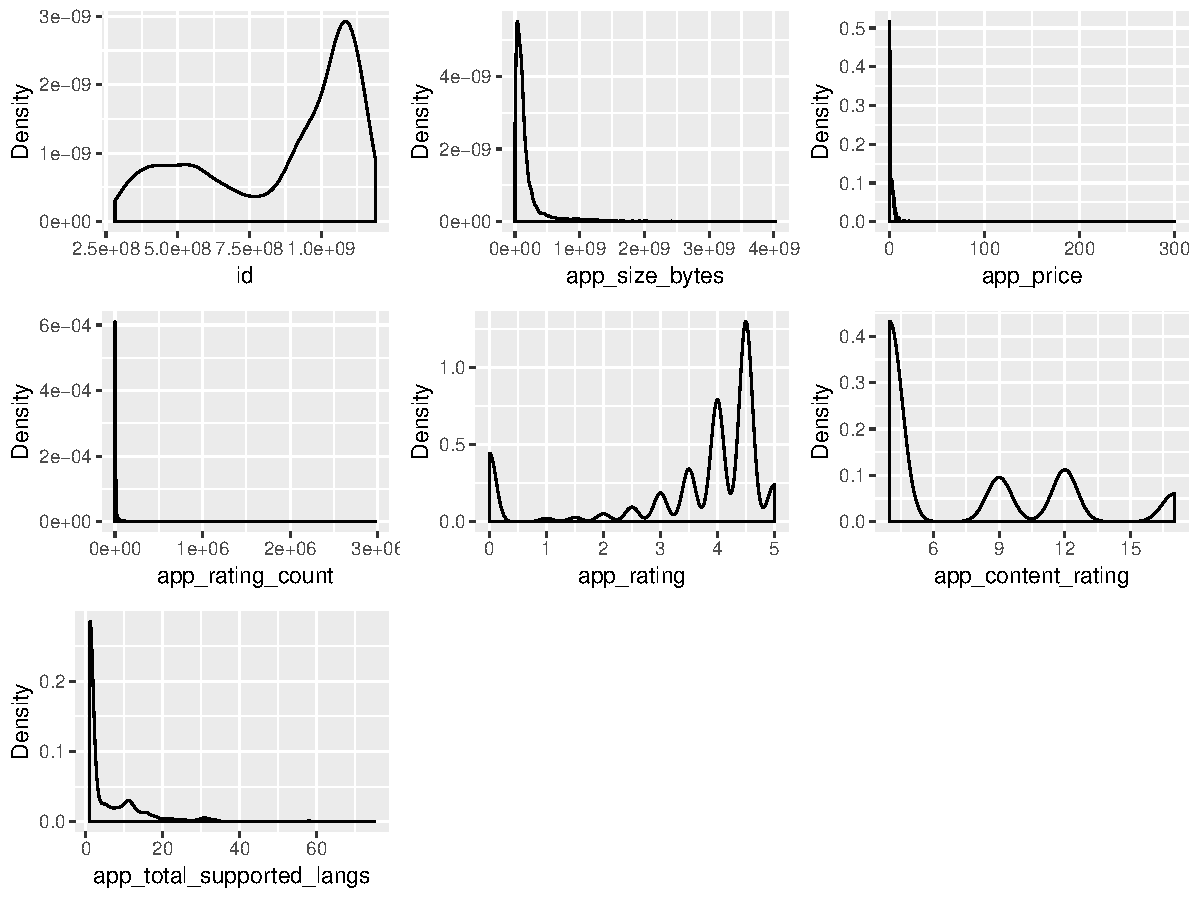
\includegraphics{Plots/analysis1-1} \end{center}
\newpage

I immediately noticed that \(\texttt{appStore\$id}\) is a a left-skewed
bimodal distribution. The ID is simply a number and won't be useful in
identifying trends in the App Store, so I moved on to other columns. The
majority of apps on the market are less than 1000MB
(\(10^9 = 1,000,000,000\) bytes). Depending on how OSXtern and other
supported platforms defines a gigabyte, you could say that most apps are
less than 1GB as well.

\begin{Shaded}
\begin{Highlighting}[]
\KeywordTok{plot_correlation}\NormalTok{(appStore[, }\DecValTok{2}\OperatorTok{:}\KeywordTok{ncol}\NormalTok{(appStore)], }\DataTypeTok{maxcat =} \DecValTok{24}\NormalTok{)  }\CommentTok{# function from DataExplorer library}
\end{Highlighting}
\end{Shaded}

\begin{center}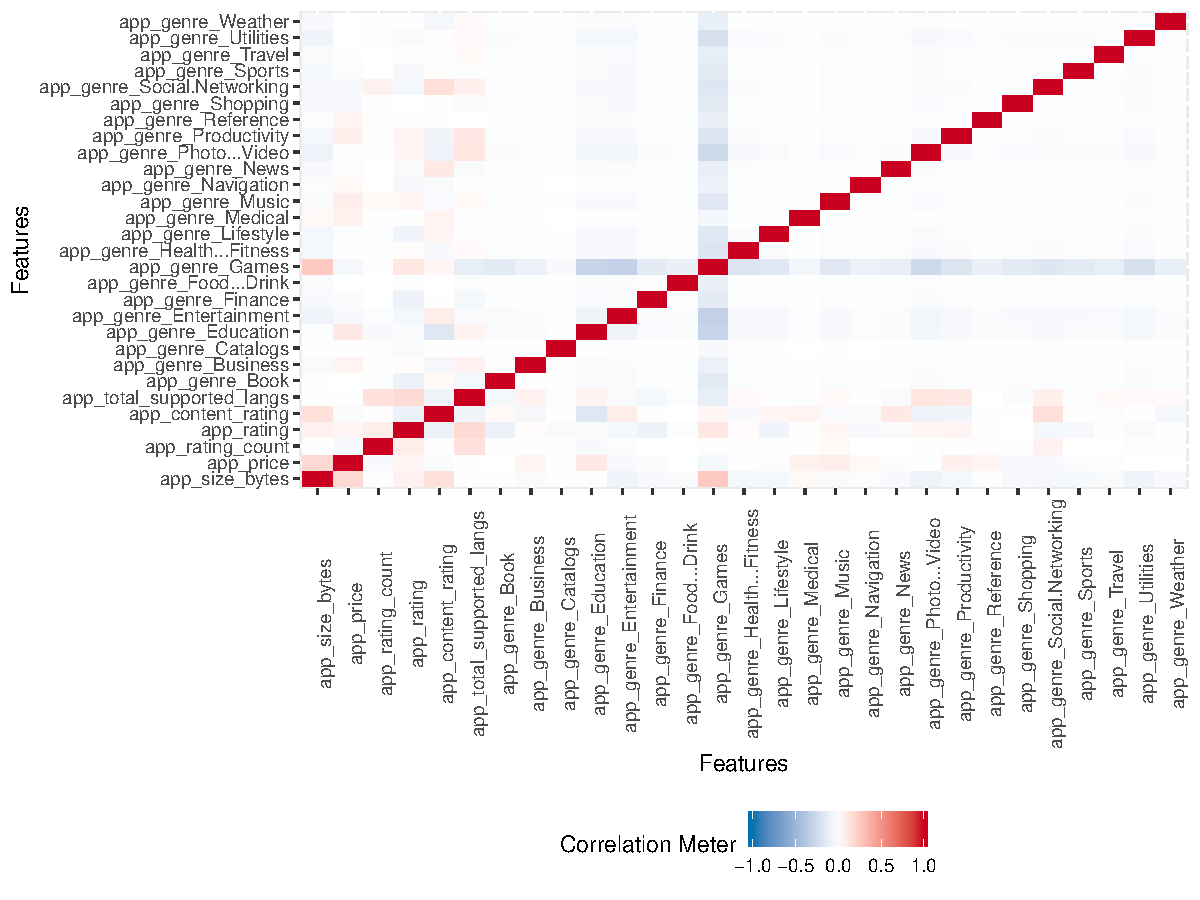
\includegraphics{Plots/analysis2-1} \end{center}

\(\textit{DataExplorer}\)'s \(\texttt{plot\_correlation()}\) function
produced a nice correlation graph of every feature. I didn't learn
anything new from it, but it confirmed that no high-correlation vector
pairs remained. The only feature not pictured is \(\texttt{app\_genre}\)
because each entry is a string. It contains nominal data; usually, I'd
assign numbers to each value before working with them, but
\(\textit{DataExplorer}\) has a visualization solution that negates the
need to first quantify the genres.

Surprisingly, app price and size have a somewhat strong correlation with
a correlation coefficient (\(r\)) of 0.18. \(r^2=0.0324\), which means
that only 3.24\% of the variation is explained by \(r\). Another strange
observation is that \(r=0.14\) for \(\texttt{app\_content\_rating}\) and
\(\texttt{app\_size\_bytes}\). Less surprising and somewhat strong
correlations include: \(\texttt{app\_rating\_count}\) vs.
\(\texttt{app\_total\_supported\_langs}\) (0.14) and
\(\texttt{app\_rating}\) vs. \(\texttt{app\_total\_supported\_langs}\)
(0.17). Finally, games tend to be bigger in size (bytes) and have higher
ratings than other apps.

\newpage

\begin{Shaded}
\begin{Highlighting}[]
\KeywordTok{plot_bar}\NormalTok{(appStore}\OperatorTok{$}\NormalTok{app_genre, }\DataTypeTok{title =} \StringTok{"Frequency of App Genres in the App Store"}\NormalTok{)}
\end{Highlighting}
\end{Shaded}

\begin{center}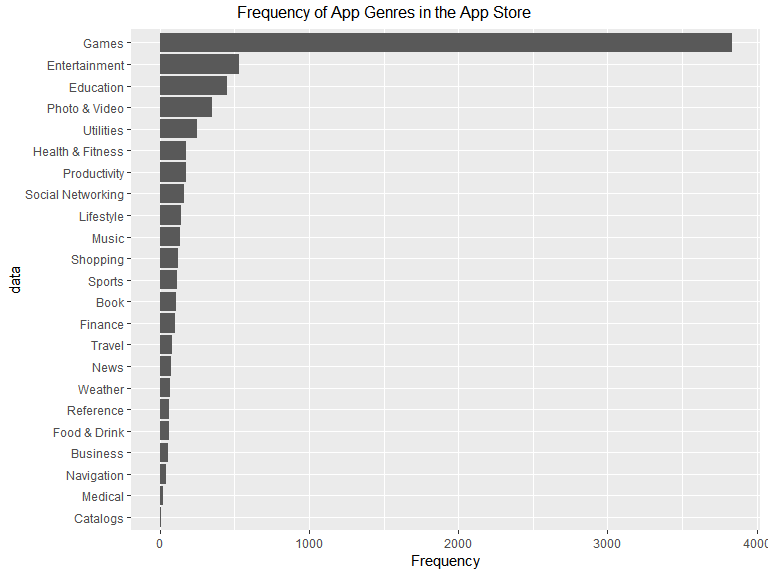
\includegraphics{Plots/analysis3-1} \end{center}

The `Games' category stands out as an outlier. The number of `Games'
apps (3832) is over 7 times greater than the number of `Entertainment'
apps (534). I created a separate dataset that contains everything but
apps labeled `Games' in case the outlier affects future observations.

\begin{Shaded}
\begin{Highlighting}[]
\NormalTok{numGames <-}\StringTok{ }\KeywordTok{sum}\NormalTok{(}\KeywordTok{grepl}\NormalTok{(}\StringTok{"Games"}\NormalTok{, appStore}\OperatorTok{$}\NormalTok{app_genre))  }\CommentTok{# most common genre}
\NormalTok{numEntertainment <-}\StringTok{ }\KeywordTok{sum}\NormalTok{(}\KeywordTok{grepl}\NormalTok{(}\StringTok{"Entertainment"}\NormalTok{, appStore}\OperatorTok{$}\NormalTok{app_genre))  }\CommentTok{# second most common genre}
\NormalTok{numGames}\OperatorTok{/}\NormalTok{numEntertainment  }\CommentTok{# ratio (7x increase)}
\end{Highlighting}
\end{Shaded}

\begin{verbatim}
## [1] 7.17603
\end{verbatim}

\begin{Shaded}
\begin{Highlighting}[]
\NormalTok{appStore.noGames <-}\StringTok{ }\NormalTok{appStore  }\CommentTok{# create copy of dataset}
\NormalTok{appStore.noGames}\OperatorTok{$}\NormalTok{app_genre[}\KeywordTok{grepl}\NormalTok{(}\StringTok{"Games"}\NormalTok{, appStore.noGames}\OperatorTok{$}\NormalTok{app_genre)] <-}\StringTok{ }\OtherTok{NA}  \CommentTok{# replace games with NA}
\NormalTok{appStore.noGames <-}\StringTok{ }\KeywordTok{na.omit}\NormalTok{(appStore)  }\CommentTok{# remove games (now NA)}
\end{Highlighting}
\end{Shaded}

\(\textbf{Xbot}\) is an assistant, so it'd best fit in the `Utilities'
category. I compared this category to its nearest competitors below:

\begin{Shaded}
\begin{Highlighting}[]
\NormalTok{numPhoto <-}\StringTok{ }\KeywordTok{sum}\NormalTok{(}\KeywordTok{grepl}\NormalTok{(}\StringTok{"Photo & Video"}\NormalTok{, appStore}\OperatorTok{$}\NormalTok{app_genre))}
\NormalTok{numUtil <-}\StringTok{ }\KeywordTok{sum}\NormalTok{(}\KeywordTok{grepl}\NormalTok{(}\StringTok{"Utilities"}\NormalTok{, appStore}\OperatorTok{$}\NormalTok{app_genre))}
\NormalTok{numHealth <-}\StringTok{ }\KeywordTok{sum}\NormalTok{(}\KeywordTok{grepl}\NormalTok{(}\StringTok{"Health & Fitness"}\NormalTok{, appStore}\OperatorTok{$}\NormalTok{app_genre))}

\NormalTok{numUtil  }\CommentTok{# number of utility apps}
\end{Highlighting}
\end{Shaded}

\begin{verbatim}
## [1] 248
\end{verbatim}

\begin{Shaded}
\begin{Highlighting}[]
\NormalTok{numPhoto }\OperatorTok{-}\StringTok{ }\NormalTok{numUtil  }\CommentTok{# distance to upper neighbor}
\end{Highlighting}
\end{Shaded}

\begin{verbatim}
## [1] 100
\end{verbatim}

\begin{Shaded}
\begin{Highlighting}[]
\NormalTok{numUtil }\OperatorTok{-}\StringTok{ }\NormalTok{numHealth  }\CommentTok{# distance to lower neighbor}
\end{Highlighting}
\end{Shaded}

\begin{verbatim}
## [1] 68
\end{verbatim}

Unlike `Games', `Utilities' is reasonably close to its neighbors. It's a
popular yet less-saturated genre with only 248 apps. \(\textbf{Xbot}\)
has a higher chance of success than any new game that comes to the app
store because it has less competition. If advertised properly, it could
very easily top the charts.

Next, I focused on the price of the apps in the dataset
(\(\texttt{appStore\$app\_price}\)). Unsurprisingly, the majority (56\%)
were free. I must admit that I'm unsure what to make of this; the naive
answer would be to make \(\textbf{Xbot}\) a free app too to achieve the
same accessibility and popularity as the others. People are more likely
to download and try a free app than pay for an app they may not enjoy
using.

\begin{Shaded}
\begin{Highlighting}[]
\KeywordTok{sum}\NormalTok{(appStore}\OperatorTok{$}\NormalTok{app_price }\OperatorTok{==}\StringTok{ }\DecValTok{0}\NormalTok{)}\OperatorTok{/}\KeywordTok{nrow}\NormalTok{(appStore)  }\CommentTok{# 56% of apps are free}
\end{Highlighting}
\end{Shaded}

\begin{verbatim}
## [1] 0.5627446
\end{verbatim}

\begin{Shaded}
\begin{Highlighting}[]
\NormalTok{appStore.prices <-}\StringTok{ }\KeywordTok{as.data.frame}\NormalTok{(}\KeywordTok{table}\NormalTok{(appStore}\OperatorTok{$}\NormalTok{app_price))  }\CommentTok{# store prices in new dataframe}
\KeywordTok{names}\NormalTok{(appStore.prices)[}\DecValTok{1}\NormalTok{] <-}\StringTok{ "Price"}  \CommentTok{# rename first dataframe vector}
\KeywordTok{plot}\NormalTok{(appStore.prices)  }\CommentTok{# plot distribution of prices}
\end{Highlighting}
\end{Shaded}

\begin{center}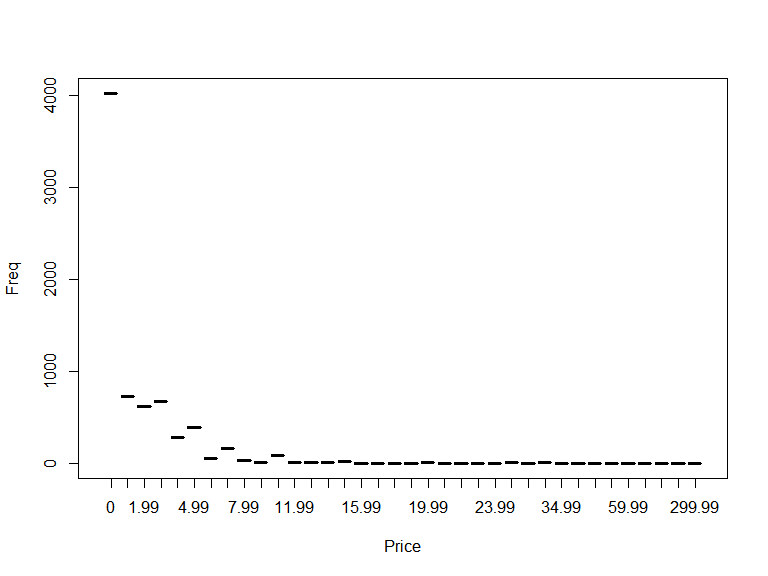
\includegraphics{Plots/analysis6-1} \end{center}

\hypertarget{conclusion}{%
\section{Conclusion}\label{conclusion}}

To make \(\textbf{Xbot}\) a success, TechPointX needs to list the app as
a ``Utility'' and consider making the app free to incite downloads. App
size and rating are positively correlated, but making an app less than
1GB is common and undoutebly expected by consumers. \(\textbf{Xbot}\)
needs to have the lowest app content rating possible to increase the
number of potential users. It would be beneficial to hire a localization
team to ensure everyone can use the app no matter the locale. The more
languages an app supports, the higher the rating according to the
dataset.


\end{document}
